%----------------------------------------------------------------------------------------
%	PACKAGES AND OTHER DOCUMENT CONFIGURATIONS
%----------------------------------------------------------------------------------------

\documentclass[letterpaper]{inzane_syllabus} % a4paper for A4

\usepackage{booktabs, colortbl, xcolor}
\usepackage{tabularx}
\usepackage{enumitem}
\usepackage{ltablex} 
\usepackage{multirow}

\setlist{nolistsep}

\usepackage{lscape}
\newcolumntype{r}{>{\hsize=0.9\hsize}X}
\newcolumntype{w}{>{\hsize=0.6\hsize}X}
\newcolumntype{m}{>{\hsize=.9\hsize}X}

\renewcommand{\familydefault}{\sfdefault}
\renewcommand{\arraystretch}{2.0}
%----------------------------------------------------------------------------------------
%	 PERSONAL INFORMATION
%----------------------------------------------------------------------------------------

\profilepic{logo.png} % Profile picture, if the height of the picture is less than that of the cirle, it will have a flat bottom. 


% To remove any of the following, you need to comment/delete the lines in the .cls file (c. line 186). Commenting/deleting the lines below will produce an error. 

%To add different lines, you will need to create the new command, e.g. \profPhone, in the .cls file c. line 76, and command to create the line in the side bar in the .cls file c. line 186

%\classname{AI for music\\and the arts} 
\classname{Creative\\computing\\and  music\\ making} 
\classnum{MUSIC 30} 

%%%%%%%%%%%%%%% PROF INFO
\profname{Carmine-Emanuele Cella}
\officehours{By appointment only} 
\office{Center for New Music and Audio Technologies (CNMAT)}
\site{http://www.carminecella.com} 
\email{carmine.cella@berkeley.edu}

%%%%%%%%%%%%%%% COURSE  INFO
\prereq{Prereq: None}
\classdays{}
\classhours{}
\classloc{CNMAT (McEnerney Hall)}

%%%%%%%%%%%%%%% LAB INFO
\labdays{}
\labhours{}
\labloc{CNMAT (McEnerney Hall) - Laptop and headphones required}

%%%%%%%%%%%%%%% TA INFO
\taAname{Alice}
\taAofficehours{Office Hrs: Tues \& Thurs 10-11a}
\taAoffice{MCZ 104}
% \taAemail{}
\taBname{James}
\taBofficehours{Office Hrs: Tues \& Thurs 3-4p}
\taBoffice{MCZ 104}
% \taBemail{}

%\about{Fish make up the largest group of vertebrates on the planet, easily outnumbering mammals, marsupials, birds, and reptiles combined. Not only are they abundant, but they've diversified into an extraordinary array of sizes, shapes, lifestyles, and habitats. You can find them in the coldest, deepest parts of the ocean, and in the hottest freshwater ponds in the desert. This course will explore fish diversity and their biology. } 


%---------------------------------------------------------------------------------------
%	 FAQs
%----------------------------------------------------------------------------------------
%to add more questions or remove this section, go to the .cls file and start with lines comment
%lines 226-250. Also comment out this section as well as line 152(ish), the command \makeSide

\qOne{Do I need to know machine learning?}
\aOne{No. The essential tools of machine learning will be introduced in the course.}

\qTwo{Do I need to know Python programming?}
\aTwo{No. All Python-based labs will be based on ready-to-use Jupyter notebooks. }

\qThree{Do I need to know Max programming?}
\aThree{No. All Max-based labs will be based on ready-to-use programs with a graphical interface.}

\qFour{How much musical knowledge is required?}
\aFour{Nothing more than an intuitive understanding of concepts such as melody or timbre. The motivation of the course is to explore tools to create and transform sound that are of general interest to all and applicable to all genres of music.}

%----------------------------------------------------------------------------------------

\begin{document}

%----------------------------------------------------------------------------------------
%	 DESCRIPTION
%----------------------------------------------------------------------------------------

\makeprofile % Print the sidebar

%----------------------------------------------------------------------------------------
%	 OVERVIEW
%----------------------------------------------------------------------------------------
\section{Overview}

 The advancements in machine learning, especially the recent breakthrough of artificial neural networks, promoted novel art practices in which computers play a fundamental role and fostered research in the field of computational creativity. Alongside other arts, music has also benefited from the development of machine learning and artificial intelligence.

 \textcolor{myCOLOR}{Music 30 (\emph{Creative computing and music making})} aims at exploring the potential that computers have to support, enhance and transform music making. The course is divided into three modules. The first module gives a general introduction to sound and presents the creative relationship between music and machine learning. The second module shows real problems in creative computing for music. The third module focuses on the connection between the society and creative computing at large. The classes are supported by labs based on state-of-the-art computational tools developed at the Center for New Music and Audio Technologies (CNMAT), UC Berkeley.

%----------------------------------------------------------------------------------------
%	 EXTRAS
%----------------------------------------------------------------------------------------

\vspace{0.5cm}
\section{Students Learn To}

%use \begin{outline} or \begin{outline}[enumerate] to create a list with subitems. 
\begin{itemize}
\item Explore synergies between human and computational creativity 
\item Use and manipulate digital tools for music creation
\item Critically evaluate computational artefacts
% \item Review a paper and provide helpful criticism to your peers' work
\item Understand the impact of creative computing on our society
\end{itemize}

%----------------------------------------------------------------------------------------
%	 READING MATERIAL
%----------------------------------------------------------------------------------------
\vspace{0.5cm} %I make liberal use of the \vspace{} command to partition and place sections just how I want them. Alter as you see fit. 
\section{Materials}

{\color{myCOLOR} Required Texts}\\
("BEN") D. Benson, \textit{Music: a mathematical offering}, freely available on author's web page, 2007.\\
("BUR") A. Burkov, \textit{The Hundred-page machine learning book}, available at a very affordable price on \url{https://leanpub.com/theMLbook} (link to external site), 2019.\\
% ("STR") G. Strang, \textit{Linear algebra and learning from data}, Wellesley Cambridge Press, 2019.\\

{\color{myCOLOR} Recommended Texts}\\
C. E. Cella, \textit{Creative computing for music and sound}, MIT Press, in preparation. \\
A. G\'eron, \textit{Hands-on machine learning with Scikit-Learn \& TensorFlow}, O'Reilly, 2017.\\
E. A. Lee, \textit{The coevolution: the entwined futures of humans and machines}, MIT Press, 2017.\\

{\color{myCOLOR} Other}\\
Music 30 will use Python/Anaconda (\url{https://www.anaconda.com}, link to external site) and Cycling’74 Max (\url{http://cycling74.com/}, link to external site) programming environments extensively during the labs. The free audio editor Ocenaudio (\url{https://www.ocenaudio.com}, link to external site) will also be used during classes. Students must have access to a laptop computer with these software packages installed and must have headphones. Students may choose to purchase Max, or alternatively there are student authorization options. Any required journal/conference articles and all the source code for the labs will be provided on \emph{bCourses}. Relevant drafts of \emph{Creative computing for music and sound} will also be distributed during the labs as lecture notes.

%----------------------------------------------------------------------------------------
%	 GRADING SCHEME
%----------------------------------------------------------------------------------------
\vspace{0.5cm}
\section{Grading Scheme}

20\% Attendance and discussion participation \\
30\% Lab assignments \\
20\% Midterm Exam \\
30\% Final Exam \\

Grades will follow the standard scale: A+ (98 to 100), A ($<$98 to 94), A-($<$94 to 90), B+ ($<$90 to 87), B ($<$87 to 83), B-($<$83 to 80), C+ ($<$80 to 77), C ($<$77 to 73), C-($<$73 to 70), D+ ($<$70 to 67), D ($<$67 to 63), D-($<$63 to 60), F ($<$60 to 0). Curving is at the discretion of the professor. 

%%%%%%%%%%%%%%%%%%%%%%%%%%%%%%%%%%%%%%%%%%%%%%%%%%%%%%%%%%%%%%%%%%%%%%%%%%%%%
%                SECOND PAGE
%%%%%%%%%%%%%%%%%%%%%%%%%%%%%%%%%%%%%%%%%%%%%%%%%%%%%%%%%%%%%%%%%%%%%%%%%%%%%

\newpage % Start a new page

\makeSide % Print the FAQ sidebar; To get rid of, simply comment out and uncomment \makeFullPage

% \makeFullPage


\vspace{0.5cm}
\section{Assignments, Exams and Make-up Policy}

Assignments will be given after each lab and they must be turned in before the next lab. They may include small closed-answer questions to be done on \emph{bCourses} and hands-on projects. There will also be a midterm  and a final, both designed as essay-based take-home exams to be written over a 72-hour period. Assignments and exams must be done individually by each student.

Make-up exams or assignments will only be allowed for students who have a substantiated excuse approved by the instructor \emph{before the due date}. Leaving a phone message or sending an e-mail without confirmation is not acceptable. Labs are mandatory.

\vspace{0.5cm}
\section{Cheating and Plagiarism}

Anyone caught cheating on a quiz or exam in this course will receive a failing grade in the course and will also be reported to the University Center for Student Conduct.

To copy text or ideas from another source without appropriate reference is plagiarism and will result in a failing grade for your assignment and usually further disciplinary action. For additional information on plagiarism and how to avoid it, see, for
example: \url{http://gsi.berkeley.edu/teachingguide/misconduct/prevent-plag.html}.

\vspace{0.5cm}
\section{Academic Integrity}

Berkeley's honor code states "As a member of the UC Berkeley community, I act with honesty, integrity, and respect for others" (\url{https://teaching.berkeley.edu/berkeley-honor-code}). The honor code is a cornerstone of our learning community and of this course. It is your responsibility to know and follow academic integrity policies. I will gladly answer any questions you have.\\

\vspace{0.5cm}
\section{Diversity and Inclusivity Statement}

I consider this classroom to be a place where you will be treated with respect, and I welcome individuals of all ages, backgrounds, beliefs, ethnicities, genders, gender identities, gender expressions, national origins, religious affiliations, sexual orientations, ability - and other visible and non-visible differences. All members of this class are expected to contribute to a respectful, welcoming and inclusive environment for every other member of the class. 

\vspace{0.5cm}
\section{Accommodations for Students with Disabilities}

If you are a student with learning needs that require special accommodation, contact the Disabled Students' Program (\url{https://dsp.berkeley.edu}), as soon as possible, to make an appointment to discuss your special needs.  Please e-mail me in order to set up a time to discuss your learning needs.

\vspace{0.5cm}
\section{Harassment and Discrimination}

The University of California strives to prevent and respond to harassment and discrimination. Engaging in such behavior may result in removal from class or the University. If you are the subject of harassment or discrimination there are resources available to support you. Please contact the Confidential Care Advocate (\url{https://care.berkeley.edu}) for non-judgmental, caring assistance with options, rights and guidance through any process you may choose. Survivors of sexual violence may also want to view the following website: \url{https://svsh.berkeley.edu}.
For more information about how the University responds to harassment and discrimination, please visit the Office for the Prevention of Harassment and Discrimination website: \url{https://ophd.berkeley.edu}.\\


%%%%%%%%%%%%%%%%%%%%%%%%%%%%%%%%%%%%%%%%%%%%%%%%%%%%%%%%%%%%%%%%%%%%%%%%%%%%%
%                COURSE SCHEDULE
%%%%%%%%%%%%%%%%%%%%%%%%%%%%%%%%%%%%%%%%%%%%%%%%%%%%%%%%%%%%%%%%%%%%%%%%%%%%%
\newpage
\makeFullPage
\section{Class Schedule}

\begin{center}
\begin{tabularx}{\textwidth}{p{2cm}p{8cm} @{\hskip 0.5cm} p{9.5cm}} %change the width of the comments by changing these cm measurements. Add/substract columns by adding/deleting p{} sections. 
\arrayrulecolor{myCOLOR}\hline
\hline 
\hline 

%%%%%%%%%%%%%%%%%%%%%%%%%%%%%%%%%%%%%%%%%%% MODULE 1
\multicolumn{3}{l}{\textbf{\textcolor{myCOLOR}{\large MODULE 1: Foundations }}} \\
\hline
  \# & Topic & Readings \\ \hline 
%%Alternatively, instead of Week #, you can do Class date for meeting
Week 1 &
Creative computing is not \ldots creative: the four \emph{P}s of creativity & F. Carnovalini and A. Rod\`a, Computational Creativity and Music Generation Systems: An Introduction to the State of the Art. Front. Artif. Intell. 3:14, 2020  \\

& & Suggested: M. A. Boden, Computer models of creativity. AI Mag. 30:23, 2009 \\

& Creative artefacts vs assisted creation: dualities in modelling creativity for the arts&  Lecture notes \\
& & R. L. De M\`antaras, Artificial Intelligence and the Arts: Toward Computational Creativity, in The Next Step: Exponential Life, 2017\\
% & &  Suggested: S. Colton, J. W. Charnley and A. Pease, Computational creativity theory: the FACE and IDEA descriptive models, in ICCC (Mexico City), 90–95, 2011 \\
\arrayrulecolor{maingray}\hline

Week 2 & Three introductory views on sound: physical, perceptual and cultural & [BEN, ch. 1.1-1.7]\\

& Introduction to musical timbre and digital signals & [BEN, ch. 7.1-7.6, appendix M]\\
\arrayrulecolor{maingray}\hline
\arrayrulecolor{maingray}\hline
\arrayrulecolor{maingray}\hline
\arrayrulecolor{maingray}\hline

Week 3 & Music without data (I): making new sounds using frequency-based representations & Lecture notes\\

& & Suggested: C. E. Cella, A geometric interpretations of signals, available on www.carminecella.com, 2015\\

& \emph{Lab (Python)}: transforming sounds and images with convolutional maps & Suggested: C. E. Cella, On room impulse response measurements with sine sweeps, available on www.carminecella.com, 2017 \\
\arrayrulecolor{maingray}\hline

Week 4 & Music without data (II): making music using rules &  S. R. Holtzman, Using Generative Grammars for Music Composition, Computer Music Journal , Spring, 1981, Vol. 5, No. 1 (Spring), pp. 51-64, 1981\\
% & & Suggested: F. Courtot, A constraint-based logic program for generating polyphonies, in Proceedings of the International Computer Music Conference, pp. 292–294, 1990 \\

&  \emph{Lab (Python)}: L-systems for melodic generation and choral harmonisation&  S. Mason and M. Saffle, L-Systems, melodies and musical structure, Leonardo Music J. 4, 31–38, 1994 \\
\arrayrulecolor{maingray}\hline
\arrayrulecolor{maingray}\hline
\arrayrulecolor{maingray}\hline
\arrayrulecolor{maingray}\hline

Week 5 & Music with data (I): making music using probabilities & Lecture notes \\

& \emph{Lab (Python)}: Markov models for text and music generation & Suggested: C. Bell, Algorithmic music composition using dynamic Markov chains and genetic algorithms, J. Comput. Sci. Coll. 27, 99–107, 2011\\
% & & J. D. Fern\'andez and F. Vico, AI methods in algorithmic composition: a comprehensive survey, J. Artif. Intell. Res. 48, 513–58, 2013 \\
\arrayrulecolor{maingray}\hline

Week 6 & Music with data (II): making music using optimisation &  Lecture notes\\
 
& \emph{Lab (Max)}: \emph{Orchidea} and computer-assisted orchestration & A. Horner and D. E. Goldberg, Genetic algorithms and computer-assisted  music composition, in ICMC, Vol. 91 (Ann Arbor, MI), 479–482, 1991 \\
& & Suggested: C. E. Cella, Orchidea: a comprehensive framework for target-based computer-assisted dynamic orchestration, Journal of New Music Research, under review, 2020 [sections 1, 2 (except 2.2.1), 4.1, 4.2, 4.10, 5]  \\
\arrayrulecolor{maingray}\hline

Week 6 & Music with data (III): making music and new sounds using neural networks & Lecture notes \\
& & [BUR, ch. 1]\\

& \emph{Lab (Python)}: \emph{Magenta NSynth}, how machine learning tools can help artists create art and music & [BUR, ch. 2] \\
\arrayrulecolor{maingray}\hline

 Week 8 & Review & Module 1 \\
 &EXAM &  MIDTERM \\
& & \\ 
 \arrayrulecolor{myCOLOR}\hline
\multicolumn{2}{l}{\textbf{\textcolor{myCOLOR}{\large MODULE 2: Problems }}} \\
\hline

Week 9 & The problem of modelling time and timbre in music &  Lecture notes \\
& &  Suggested: H. C. Crayencour, C. E. Cella, Learning, probability and logic: towards a unified approach for content-based Music Information Retrieval, Frontiers in Digital Humanities, April 2019 \\


% & & Suggested: S. Dieleman, A.  van den Oord,  and K. Simonyan, The challenge of realistic music generation: modelling raw audio at scale, in Advances in Neural Information Processing Systems 31, eds S. Bengio, H. Wallach, H. Larochelle, K. Grauman, N. Cesa-Bianchi, and R. Garnett (Red Hook, NY: Curran Associates,
% Inc.), 7989–7999, 2018 \\

& \emph{Lab (Max and Python)}: granular synthesis and \emph{AudioGuide} & B. Hackbarth, N. Schnell and D. Schwarz, Audioguide: A Framework For Creative Exploration Of Concatenative Sound Synthesis, IRCAM research report, 2011. \\

\arrayrulecolor{maingray}\hline

Week 10 & The problem of musical style transfer (I): introduction & Lecture notes \\

% & L. A. Hiller and L. M. Isaacson, Musical composition with a high-speed
% digital computer. J. Audio Eng. Soc. 6, 154–160, 1958 \\
% & & D. Cope, Recombinant music: using the computer to explore musical style, Computer 24, 22–28, 1991 \\
% & &  Suggested: G. A. Wiggins, Computer models of musical creativity: a review of computer models of musical creativity by David cope. Literary Linguist. Comput. 23, 109–116, 2007 \\

&   \emph{Lab (Max)}: spectral freeze and cross-synthesis, a prelude to musical style transfer & [BEN, 2.1-2.2, 2.13, 2.15, 2.18] \\
\arrayrulecolor{maingray}\hline

Week 11 & The problem of musical style transfer (II): approaches based on probabilities and unsupervised methods & [BUR, ch. 9] \\

& & Suggested: C. E. Cella, Sound-types: a new framework for symbolic sound analysis and synthesis, ICMC, Huddersfield, United Kingdom, 2011 \\

&\emph{Lab (Python)}: sound-types, a first step towards musical style transfer & Suggested: C. E. Cella and J.J. Burred, Advanced sound hybridizations by means of the theory of sound-types, ICMC, Perth, Australia, 2013 \\

\arrayrulecolor{maingray}\hline
Week 12 & The problem of musical style (III): approaches based on deep learning &  [BUR, ch. 6] \\
% & &  L. Gabrielli, C. E. Cella, F. Vespertini, D. Droghini, E. Principi and S. Squartini, Deep Learning for Timbre Modification and Transfer: an Evaluation Study, AES 144th, Milan, 2018 \\
& & Suggested: J. P. Briot, and F. Pachet, Deep learning for music generation: challenges and directions, Neural Comput. Appl. 32, 981–993, 2018 \\

&\emph{Lab (Python)}: an algorithm for universal musical style transfer &  Suggested: Noam Mor, Lior Wolf, Adam Polyak, Yaniv Taigman, A universal music translation network, ICLR, 2019 \\
& & \\ 

\arrayrulecolor{myCOLOR}\hline
\multicolumn{2}{l}{\textbf{\textcolor{myCOLOR}{\large MODULE 3: Connections}}} \\
\hline
\arrayrulecolor{maingray}\hline

Week 13 & Extending the techniques to other arts: image style transfer & Lecture notes \\
& & Suggested: L. A. Gatys, A. S. Ecker, M. Bethge, Image Style Transfer Using Convolutional Neural Networks, CVPR, 2016 \\ 
&Accountability: how to evaluate creative outcomes & C. Ariza, The Interrogator as Critic: The Turing Test and the Evaluation of Generative Music Systems, Computer Music Journal 33:2, 48-70, 2009  \\
& & S. Colton, Creativity versus the perception of creativity in computational systems, in AAAI Spring Symposium: Creative Intelligent Systems Vol. 8 (Palo Alto, CA), 7, 2008 \\
& & Suggested: A. Jordanous, A standardised procedure for evaluating creative systems:
computational creativity evaluation based on what it is to be creative. Cogn. Comput. 4, 246–279, 2012 \\
\arrayrulecolor{maingray}\hline

Week 14 & On the aesthetics of computational creativity & P. Galanter, Computational aesthetic evaluation: past and future, in Computers and Creativity, eds J. McCormack and M. d’Inverno (Berlin; Heidelberg: Springer), 255–29, 2012  \\

& Social impact of assisted creation & D. K. Simonton, Creativity: cognitive, personal, developmental, and social aspects. Am. Psychol. 55:15, 2000 \\
& & Suggested: M. I. Stein, Creativity and culture. J. Psychol. 36, 311–322, 1953 \\
\arrayrulecolor{maingray}\hline

Week 15 & Review & Modules 2 and 3\\

& EXAM & FINAL \\
\arrayrulecolor{myCOLOR}\hline
\hline 
\hline 
\hline 
\end{tabularx}
\end{center}


% \vspace{0.5cm}
% \section{The five pillars of creative computing}

% \begin{center}
%   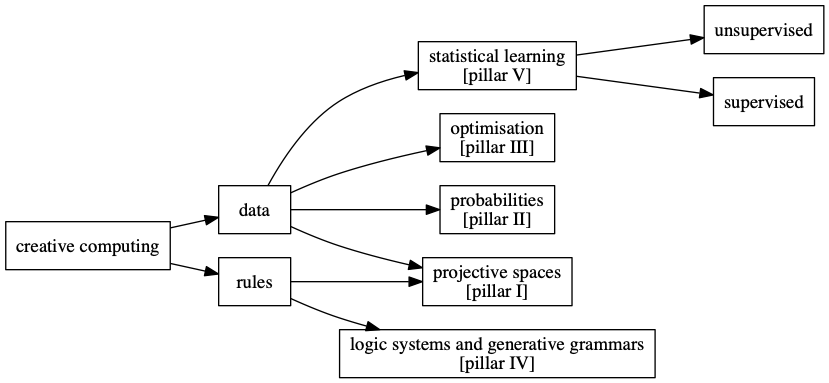
\includegraphics[scale=.5]{creative_pillars.png}  
% \end{center}

% \newpage
\vspace{0.5cm}
\section{Emergency procedures (McEnerney Hall)}

Your emergency evacuation assembly area is the steps directly across Arch St. leading to the Pacific School of Religion.
In the event of an emergency please follow instructions from your instructor and CNMAT staff.
Take note of emergency procedures posted in your classroom. If the fire alarm is sounding, exit the building immediately. In the event of an earthquake, duck when possible and hold in place, covering your head with your arms, a binder or your laptop. Then exit the building when the shaking stops.

EMERGENCY SERVICES:
\begin{itemize}
\item UC Police and all emergencies number from campus phones: 911
\item UC Police and all emergencies number from cell phones: (510) 642-3333
\item UC Police non-emergency number: (510) 642-6760
\end{itemize}
RESTROOM ACCESS: 
Restrooms at 1750 Arch Street are available to all genders.


\end{document} 



